\chapter{Theorie}

\section{Grundlagen MRT}
Die Magnetresonanztomographie (MRT) ist ein Bildgebendes Verfahren, bei der keine ionisierender Strahlung eingesetzt wird.
Dadurch gibt es keine Strahlenbelastung für Patientinnen und Patienten und die Untersuchung kann beliebig oft wiederholt werden.
Die MRT wird zur Darstellung von morphologischen Strukturen und zur Abbildung funktioneller Prozesse verwendet.
Das MRT-Gerät besteht aus einem zylinderförmigen, supraleitenden Magneten, der ein homogenes Hauptmagnetfeld $B_0$ erzeugt. %Shimming optional
In der klinischen Anwendung liegt die Magnetfeldstärke bei $\qty{1.5}{T}$ - $\qty{3}{T}$.~\cite{Schlegel}
Die Kernteilchen besitzen einen magnetischen Moment $\vec{m}$, aufgrund dessen das sie um ihre eigene Achse, mit der Lamorfrequenz 
\begin{equation}
    \omega_0 = \gamma \cdot B_0
\end{equation}
präzedieren. $\gamma$ beschriebt dabei das Gyromagnetische Verhältnis, welches Materialabhängig ist.
Die magnetischen Momente des Kerns summieren sich und es entsteht eine gesamt Magnetisierung $\vec{M}$ des Atoms. Befinden sich diese Atome im Magnetfeld,
richten sich die Spins der Kernteilchen parallel und antiparallel nach dem Magnetfeld aus. Sie befinden sich im thermischen Gleichgewicht.
Bei Atomen mit einer geraden Anzahl an Kernteilchen heben sich beim aufsummieren die magnetischen Momente auf und besitzen somit keine
Magnetisierung. 
Da die Magnetisierung notwendig für die Messung eines Signals im MRT ist, können nur Atome mit einer ungeraden Anzahl an Kernteilchen gemessen werden.
Am häufigsten wird zur Messung Wasserstoff verwendet, da dies mit ca. $\qty{80}{\%}$ am häufigsten im Menschlichen Körper vorkommt.
Mittels eines Hochfrequenzsignals (HF) werden die Spins um einen Winkel
\begin{equation}
    \alpha = \gamma \cdot B_1 \cdot T 
\end{equation}
gekippt. Dabei entspricht $B_1$ dem Anregungsimpuls und $T$ die Zeit des HF-Impulses.
Die Frequenz des HF-Signals entspricht der Lamorfrequenz des Atoms, damit es zur Resonanz kommt. 
Beim Ausschalten des Signals, relaxieren die Kernteilchen zurück in ihre Gleichgewichtsmagnetisierung. 
Dabei wird zwischen T1-Relaxation und T2-Relaxation unterschieden. Mittels dieser Unterscheidung und der Einstellung der Echozeit $T_E$ und 
Repetitionszeit $T_R$, sind die Bilder unterschiedlich Gewichtet.
Die Repetitionszeit beschreibt die Zeit zwischen der Verwendung zweier HF-Impulse und die Echozeit der zeitliche Abstand zwischen dem Anregungsimpuls und der Auslesung des Signals. 
Anhand der Gewichtungen entstehen unterschiedliche Kontraste.
Durch die veränderten Magnetisierung kommt es zur Induktion einer Spannung, die mittels einer Spule gemessen wird.


Bei der T1- Relaxation wird die Längsmagnetisierung betrachtet, welche mit der Zeit zunimmt.
Diese lässt sich durch 
\begin{equation}
    M_z(t) = M_z(0) (1 - e^{-\frac{t}{T_1}})
\end{equation}
% Bild 
Zur Messung des Signals, wird der Zeitpunkt $T_1$, nach der Anregung bestimmt, bei dem $\qty{63}{\%}$ der Magnetisierung wiederhergestellt wurde.~\cite{Pollmann}\\
Bei der T1 Gewichtung, sind $T_R$ und $T_E$ kurz eingestellt und zusätzlich gilt das $T_E \ll T_2$.
Fett und Muskeln werden bei dieser Gewichtung hell dargestellt und Liquor dunkel.~\cite{Schlegel}

Die T2-Relaxation beschreibt die Quermagnetisierung, welche mit der Zeit abnimmt, da die Spins dephasieren und somit das Signal zerfällt.
Dieser Signalzerfall wird als "Free Induction Decay" (FID) bezeichnet.~\cite{Dössel}
Die Magnetisierung wird durch die Formel
\begin{equation}
    M_{xy}(t) = M_{xy}(0) e^{-\frac{t}{T_2}} 
\end{equation}
beschrieben.
Zum Zeitpunkt $T_2$, wenn die transversale Magnetisierung auf $\qty{37}{\%}$ abgefallen ist, wird das Signal aufgenommen.~\cite{Pollmann}
Für T2-Gewichtete Bilder gilt, dass $T_R \gg T_1$ und sowohl $T_R$ als auch $T_E$  lang eingestellt werden. 
Bei dieser Gewichtung wird Liquor hell dargestellt und Fett und Muskeln dunkel.~\cite{Schlegel} 
Aufgrund von Inhomogenitäten im Hauptmagnetfeld, kommt es zu einem schnelleren Signalzerfall. Dies wird bezeichnet als T2* Relaxation.~\cite{Dössel}\\


Für die Erstellung des Bildes, benötigt es die drei Gradientenspulen $G_z$, $G_y$ und $G_x$. Die Anordnung der drei Spulen 
ist in Abbildung \ref{fig:an Grad} abgebildet.
\begin{figure}[htbp]
  \centering
  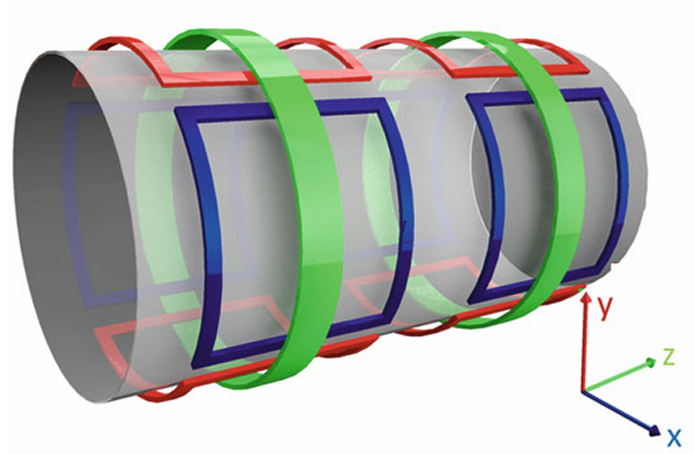
\includegraphics[scale=0.5]{/nfs/homes/sdreyer/Digit-Classification-Pytorch/tudothesis-main/content/abbildungen/Anordnung Gradientenspulen.png}
  \caption{Anordnung der Gradientenspulen.\cite{Schlegel}}
  \label{fig:an Grad}
\end{figure}
Durch das schalten der Gradienten kommt es zur Überlagerung mit dem Magnetfeld, wodurch die Codierung des Bildes möglich ist.
Der Gradient in z-Richtung wird für die Einstellung der Schichtdicke verwendet. 
Zur Frequenzcodierung wird der Gradient $G_x$ geschaltet, wodurch sich die Lamorfrequenzen entlang des Gradienten verschieben.
Mittels des Gradienten $G_y$ werden die Spins in ihrer Phase verschoben.
Durch die Verschiebung der Frequenz und Phase ist die Ortscodierung möglich und die Aufnahme eines Bildes im k-Raum.
Durch die Fouriertransformation werden die Informationen in den Ortsraum transformiert
.~\cite{pabst2013}


\section{Maschinelles Lernen}



\subsection{Neuronales Netzwerk}

Aufbau
    weights 
training: loss fkt reduzieren
Hyperparameter
Aktivierungsfunktion 
\subsection{Convolutional Neural Network}

Aufbau
